\chapter{Experiment Characterisation}
\label{ch:Characterisation}
\minitoc


    Before we can proceed with our planned experiments involving the motion and
    spin of the atoms, the apparatus must be characterised. This characterisation
    serves two purposes: it allows us to benchmark the performance of our system
    against state-of-the-art results, and it reveals any current limitations
    that must be addressed before we can successfully carry out the experiments.

\section{Quadrupole Transitions}
\label{sec:Transitions}
% Main points:
    % All visible motional modes on large detuning scan at $5$~G. 
    % Can compare when have all quadrupole transitions available or when we selectively omit transitions via polarisation.
% Pre reqs:
    % 5 G field
    \begin{figure}
        \vspace*{-0.5cm}
        \begin{center}
        \noindent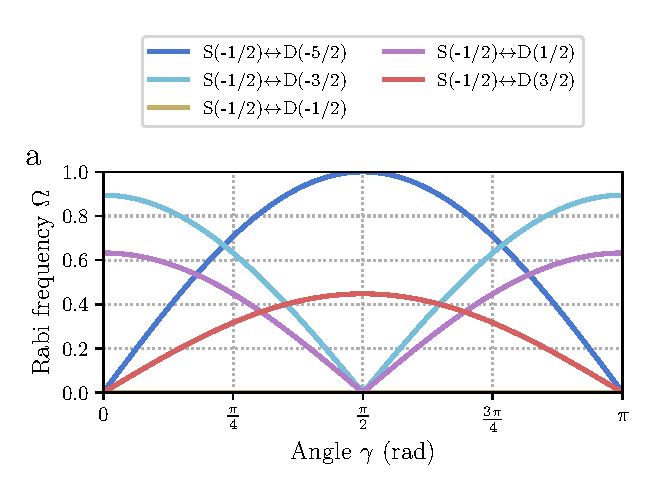
\includegraphics[width=0.65\linewidth]{
            figures/pdf_figure/qp_gamma.pdf
            }
        \vspace*{-0.5cm}
        \noindent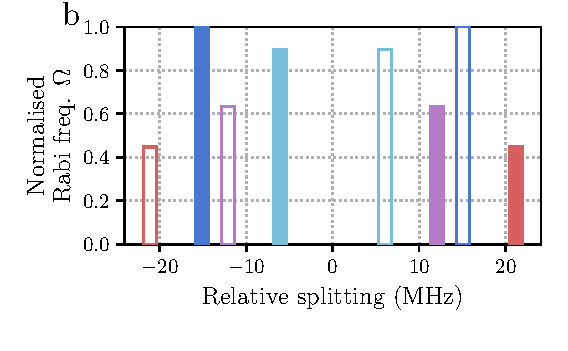
\includegraphics[width=0.65\linewidth]{
            figures/pdf_figure/qp_transition_spectrum_0.25.pdf
            }
        \vspace*{-0.5cm}
        \noindent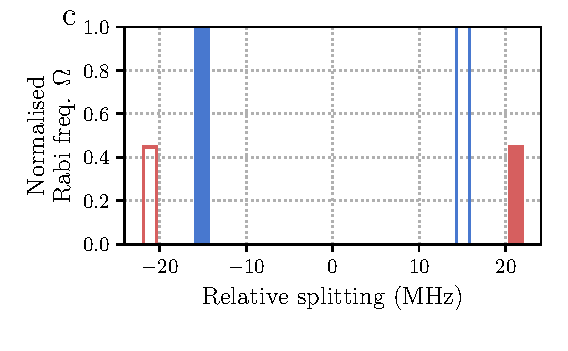
\includegraphics[width=0.65\linewidth]{
            figures/pdf_figure/qp_transition_spectrum_0.50.pdf
            }
        \end{center}
        \vspace*{-0.5cm}
        \caption{
            Normalised quadrupole Rabi frequencies, $\Omega$, and frequency splittings for the $4S_{1/2} \leftrightarrow 3D_{5/2}$ Zeeman sublevels in \ca. Solid bars correspond to transitions with lower state $4S_{1/2},~m_j = -1/2$, while open bars correspond to transitions with lower state $4S_{1/2},~m_j = +1/2$.
            \textbf{a)} Relative Rabi frequencies as angle $\gamma$ between the polarisation vector and the magnetic field is varied. The k-vector of the light is assumed to be perpendicular to the B-field.
            \textbf{b)} Relative frequency splittings and strengths when $\gamma = \pi/4$. At this angle, all transitions are accessible apart from those with $\Delta m_j = 0$. This is the polarisation chosen for our initial experiments to allow access to all transitions for characterisation.
            \textbf{c)} Relative frequency splittings and strengths when $\gamma = \pi/2$. This is the polarisation chosen for the current and future experiments to reduce the number of transitions which can cause off-resonant interactions when the qubit defined by $4S_{1/2},~m = -1/2 \leftrightarrow 3D_{5/2},~m' = -5/2$ is used.
            }
        \label{fig:quadrupole}
    \end{figure}

    The \ca ion has a rich level structure, shown in figure~\ref{fig:ion}, with many accessible quadrupole transitions $4S_{1/2}\leftrightarrow 3D_{5/2}$. The quadrupole transition is ideal for use as a qubit due to the long-lived metastable level~\cite{barton_measurement_2000}, and the ability to optically couple the transition via a laser. As mentioned in section~\ref{sec:Narrow Line Width 729 Laser}, the 729-nm beam is used for this purpose. By selecting the appropriate frequency of the 729-nm beam, qubit operations such as state preparation (section~\ref{sec:SPAM}) and single qubit gates (section~\ref{sec:Randomised Benchmarking}) may be driven, or by setting the detuning such that a motional sideband is near resonance, to couple the spin and motional degrees of freedom (section~\ref{sec:Spin-Dependent Forces}). Here, we discuss which quadrupole transitions are used, and the rationale behind their choice.\\ 
    Zeeman splitting of the $4S_{1/2}$ and $3D_{5/2}$ states leads to 2 and 6
    non-degenerate sublevels, respectively. Due to the magnetic field strength of 5.4~G (section~\ref{sec:Magnetic Field}),
    the $S$-levels are split by $\sim$15~MHz, and the $D$-levels by $\sim$9~MHz.
    This splitting is considerably larger than both the natural linewidth of the
    729-nm transition ($\sim$Hz), and the Ti:Sapph laser linewidth (<1~kHz), meaning the transitions can be 
    selectively addressed by frequency tuning of the laser. There is some freedom in choosing which of these 10 possible (with $\Delta m_j \leq 2$) quadrupole transitions we define as our qubit. Each transition has a varying coupling strength, here denoted by the relative Rabi frequency, $\Omega$, depending on the polarisation and $k$-vector of the interacting light. Here, we describe the rationale for our qubit choice of $4S_{1/2},~m = -1/2 \leftrightarrow 3D_{5/2}, ~m' = -5/2$.\\
    % Cite Gulde Thesis
    \mccorrect{XXX here change to bullet points of requirements for ``good qubit'' and do not go into details on cooling} We want excellent sideband cooling efficiency as we plan to use our motional modes considerably. For time-efficient sideband cooling, section~\ref{sec:Cooling}, a ``closed-cycle'' transition is required. ``Closed-cycle'' here means that after one cycle of sideband cooling, the final electronic state returns with high probability back to the initial electronic state. When using such a closed-cycle transition, the next sideband pulse can be run immediately, without having to state prepare the spin again. If the $4S_{1/2},~m = -1/2$ state is initially prepared, then the only closed-cycle transition is $4S_{1/2},~m = -1/2 \leftrightarrow 3D_{5/2},~m' = -5/2$. Therefore this transition must be accessible, however it does not neccessarily need to be the defined qubit transition. \\
    To further narrow down our choice, we recognise the benefit in limiting the number of addressable transitions to reduce the effect of unwanted off-resonant interactions. Figure~\ref{fig:quadrupole} $a$, shows the normalised Rabi frequencies of each transition as the angle $\gamma$ between polarisation vector and B-field is varied, while figure~\ref{fig:quadrupole} $b$, shows the relevant frequency splitting of the transitions at $\gamma = \pi/4$. These plots are for light with k-vector perpendicular to B-field, as the 729-nm addresses the ion through the main objective lens (see section~\ref{sec:Vacuum System}). This geometry suppresses transitions with $\Delta m_j = 0$. In figure~\ref{fig:quadrupole} $c$, it can be seen that at $\gamma = \pi/2$, the normalised Rabi frequency of the
    $4S_{1/2},~m = -1/2 \leftrightarrow 3D_{5/2},~m' = -5/2$ transition is maximised, while
    minimising the Rabi frequencies of all other transitions, apart from
    $4S_{1/2},~m = -1/2 \leftrightarrow 3D_{5/2},~m' = +3/2$.
    It is worth noting that access to transition $4S_{1/2},~m = +1/2 \leftrightarrow 3D_{5/2},~m' = -3/2$ is useful for state preparation, as it allows us to optically pump from $m = +1/2$ into $m = -1/2$ ground-state. \\
    If polarisation $\gamma = \pi/2$ is selected, now there are only two choices for qubit transition. This choice is simple as $4S_{1/2},~m = -1/2 \leftrightarrow 3D_{5/2},~m' = -5/2$ has both the larger Rabi frequency, and the lower magnetic field sensitivity, $-2.80$~MHz/G, compared to the $4S_{1/2},~m = -1/2 \leftrightarrow 3D_{5/2},~m' = +3/2$ transition, which has a magnetic field sensitivity of $+3.92$~MHz/G.\\
    

\section{Spin}
\label{sec:Spin}
    Discrete variable quantum computing consists of manipulating many two-level
    systems, which we refer to either as spins, or qubits. In this section 
    the methods used to maniplate these spins are described, and their
    performances are benchmarked.\\
    XXX We are interested in state prep, gates, measurement.
    Tools are Rabi, Ramsey.

\subsection{Rabi and Ramsey Scans}
\label{sec:Rabi and Ramsey Scans}
% Main points:
    % The ion is a sensor!
    % Method for Rabi and Ramsey scans
    % Mention changing polarisation to select certain transitions
    % Long Rabi flop
    % Likely reason for flop damping
    % Measuring detuning using Ramsey scan
% Pre reqs:
    % 729 system
    % Available Quadrupole transitions

% XXX read Christa's description here. Use equations, bullet points, and pulse sequence diagrams to simplify the descriptions.

    \begin{figure}
        \begin{center}
        \noindent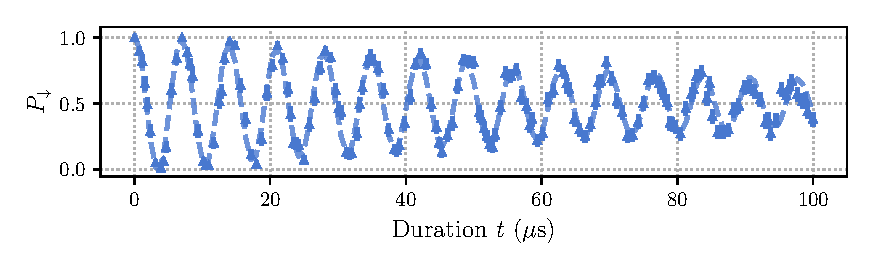
\includegraphics[width=\linewidth]{
            figures/pdf_figure/long_flop.pdf
            }
        \end{center}
        \caption{Long duration, $t$, Rabi flop on the qubit transition. Estimated probability of being in \mccorrect{XXX change all bra and kets to remove odd space}$|\downarrow\rangle$, $P_\downarrow$, at each time step using 200 individual experimental shots. Fitted dotted line using decaying oscillations model. Extracted Rabi frequency $\Omega/2\pi = 0.0716(1)$~MHz, and decay rate $\lambda = 0.0107(7)$~\unit{\per\us}\mccorrect{XXX change all units to siunitx}. 
            }
        \label{fig:Long Flop}
    \end{figure}

    Here we briefly describe the method in which the Rabi frequencies and single qubit gate durations are extracted.\\
    Access to $\pi/2|_x$-pulses is required for constructing the universal spin gate set~\cite{}. This single qubit gate is achieved by square pulses of 729-nm light. To roughly calibrate the required pulse length, extended oscillations are fitted using a damped oscillation model,
    \begin{equation}
        P_{\downarrow} = \frac{1 + e^{-\lambda t} \cos(2 \Omega t)}{2},
    \end{equation}
    where $\lambda$ is the decay rate, and $\Omega$ is the Rabi frequency.\\
    Figure~\ref{fig:Long Flop} shows one such ``flop'' with 1~mW of power-stabilised light, with a beam radius of $\sim 15 ~\mu$m at the ion. A Rabi frequency of $\Omega/2\pi = 0.0716(1)$~MHz and
    decay rate $\lambda = 0.0107(7)~1/\mu$s is found. From this a $\pi/2$ time of 1.7~$\mu$s can be estimated (note, this is on the $4S_{1/2},~m_j = -1/2 \leftrightarrow 3D_{5/2},~m_j = -3/2$ transition, which was used prior to optimising the 729-nm polarisation, see section~\ref{sec:Transitions} for more details).\\
    The damping is likely due to a combination of out-of-Lamb-Dicke effects, and laser phase noise. The out-of-Lamb-Dicke effects are due to on-resonant terms proportional to $O(\eta^2 n)$ in the full Lamb-Dicke expansion, which may not be negligible when all modes are not cooled to their ground state. As we have not yet measured all the mode temperatures after Doppler cooling, and we have not yet characterised the laser phase noise, we do not know their relative contributions to the observed decay.\\
    \mccorrect{XXX this section is unclear, either remove or reformat.} To further improve the estimate for the $\pi/2$ pulse length, the ramping time due to electronic control and AOM rise times must be accounted for. This is done by applying odd multiples of the roughly calibrated $\pi/2$ pulses consecutively, and optimising pulse durations such that the final population measurement corresponds to the Z-basis superposition state, $P_{\downarrow}= 0.5$, with $P_\downarrow = |\langle \downarrow | \psi_s \rangle|^2$, and $\psi_s$ is the qubit state. \\
    To measure the detuning of the 729-nm laser, Ramsey scans are performed.
    The qubit is first prepared in $|\downarrow\rangle = 1$, next a $\pi/2|_y$-pulse is applied to prepare the $|+\rangle$ superposition. There is some delay for time $t$, and then a second
    $\pi/2|_y$-pulse is applied. If the 729-nm is on resonance with the qubit transition, then effectively a $\pi$-pulse is performed, and the final population in $P_\downarrow$ will be 0. If the 729-nm is off-resonant, then the final population will be given by,
    \begin{equation}
        P_{\downarrow} = \frac{1+\cos(\Delta t)}{2},
    \end{equation}
    where $\Delta$ is the detuning of the laser from resonance.
    The time $t$ can be varied to increase the sensitivity to frequency offsets, and the $\Delta$ offset can be fed back to calibrate the set laser frequency. \\


    % 1 mW 729-nm laser -> Fit out pi/2, pi, 2pi pulses. We are using square pulses.


\subsection{Spin Coherence Times}
\label{sec:Coherence}
% Main points:
    % Quote coherence times comparing:
        % Mumetal box panels
        % Transitions with diff mag sensitivity
        % FNC/ no-FNC
% Pre reqs:
    % MuMetal box
    % Available transitions
    % 729 laser system

    Individual gate fidelities are ultimately limited by the loss of coherence
    between the the two qubit states. This can be caused either by dephasing or
    the natural lifetime of the $3D_{5/2}$ level. For our qubit, a lifetime limited coherence time of $\tau =
    1.1$~s~\cite{barton_measurement_2000} is expected. 
    In practise coherence times are dominated by dephasing, due to imperfect
    tracking of laser frequency and magnetic field drifts.  In characterising
    the spin coherence times, we hope to explore both the efficacy of the
    magnetic shielding surrounding the ion trap, as well as the stability of the
    729-nm laser. \\
    The spin coherence times are measured by performing Ramsey experiments.
    Contrary to the Ramsey experiments described in section~\ref{sec:Rabi and Ramsey
    Scans}, we are not interested in measuring phase accumulated over time, $t$.
    Instead, the decay in Ramsey contrast over increasing delay time is measured. As such, the phase $\phi$ of the final
    $\pi/2|_\phi$-pulse is scanned, and the contrast of the resulting fringe is measured.
    Figures~\ref{fig:coherence_times} show examples of such a scan. \mccorrect{XXX Figures not added yet.}\\
    To find the cause of the decaying contrast, the laser and
    magnetic field noise contributions can be isolated. This is done by redefining the quadrupole qubit with
    varying magnetic field sensitivity transitions. Any difference in coherence
    times measured between these transitions will be due to magnetic field
    sensitivity differences exclusively. \\
    Figure~\ref{fig:coherence_times} shows the suppression of magnetic field noise due to the MuMetal shielding. \\
    \mccorrect{XXX I dont have the data I want for this story yet.}


\subsection{State Preparation and Measurement}
\label{sec:SPAM}
% Main points:
    % Method of preparation via optical pumping
    % Readout characterisation with NA 0.6 lens
    % Compare readout histograms of fast 30 us readout to Doppler cold 100 us readout
    % Quote state prep error (back this from RBM + measurement histograms)
% Pre reqs:
    % Laser systems powers
    % 729 system
    % Available transitions
    % pi-pulses

% XXX See Machej section on state prep. Mention if we are pulsed or coninuous.
    \begin{figure}
        \begin{center}
        \noindent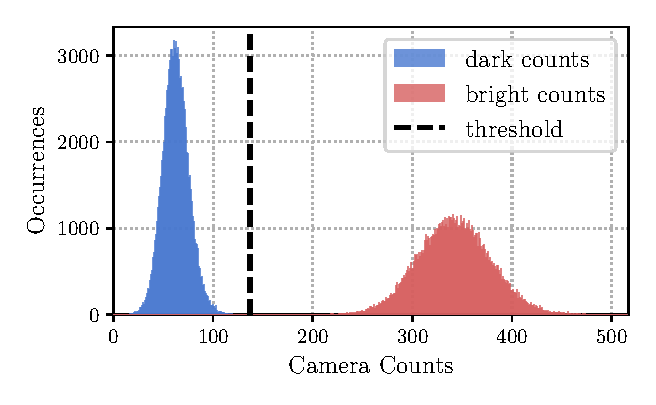
\includegraphics[width=0.75\linewidth]{
            figures/pdf_figure/readout_hist.pdf
            }
        \end{center}
        \caption{
            Readout histogram with 100,000 individual measurements for bright (red) and dark (blue) populations. The camera counts are presented as a histogram and fitted to Gaussian distributions to calibrate a threshold for discerning if the ion is bright or dark with the lowest probability for false measurement. Dark counts are mainly due to 397-nm light scattered from the nearest trap electrodes. With 100~$\mu$s readout time, and laser parameters set to Doppler cooling parameters, a threshold count of 137 photons is found, giving an expected statistical error of $6\times 10^{-9}$ given the fitted Gaussians. %Gaussian dark: mean = 62, $\sigma$ = 13. Gaussian bright: mean = 341, $\sigma$ = 36.
            }
        \label{fig:readout_histogram}
    \end{figure}

    To utilise two levels of the ion as a qubit, the ion must be able to be 
    selectively prepared into one of the Zeeman levels of the ground
    state. As mentioned in section~\ref{sec:Magnetic Field}, the fixed B-field is 5.4~G, leading to a splitting between the Zeeman
    levels of less than 21~MHz, the natural linewidth of the 397-nm transition.
    This means the state cannot be optically pumped using the 397-nm frequency selectivly.
    Further, due to the constraint of beam geometry from the in vacuum optics, see section~\ref{sec:Vacuum System},
    the state cannot be prepared using polarisation selectivity of the 397-nm transition. Instead,
    the narrow line width 729-nm laser may be used on resonance with the $4S_{1/2},~ m_j = +1/2 \leftrightarrow 3D_{5/2},~m_j = -3/2$ transition, and the 854-nm
    deshelving laser on resonance, to optically pump into the $m_j = -1/2$
    Zeeman level defined as the qubit ground state. \\
    \begin{table}
        \begin{center}
        \begin{tabular}{|c|l|}
            \hline
            Parameter & Value \\
            \hline
            397-nm laser power & 3~$\mu$W, $1\times I_{\rm SAT}$ \\
            397-nm laser detuning & -17.5~MHz\\
            866-nm laser power & 15~$\mu$W, $\sim 70\times I_{\rm SAT}$\\
            866-nm laser detuning & 0~MHz \\
            Doppler cooling duration & 1~ms\\
            Readout duration & 100~$\mu$s \\
            Camera threshold & 137 counts \\
            \hline
        \end{tabular}
        \end{center}
        \caption{
            Experimental parameters used for Doppler cooling and state-selective fluorescence of the ion. 
            }
        \label{tab:397_parameters}
    \end{table}
    To measure the qubit state, the 397-nm and 866-nm lasers
    are applied for 100~\unit{us}, and the scattered 397-nm photons are counted using a camera (see section~\ref{sec:Imaging System}). From the level diagram shown in
    figure~\ref{fig:ion}, it can be seen that upon turning on the 397-nm
    laser, if the qubit is in $|\downarrow\rangle$, photons will be scattered, and if the qubit is in
    $|\uparrow\rangle$, then no photons will be scattered. 
    \mccorrect{XXX rephrase next line:} To optimise the fidelity of
    measurement, it is ensured that the signal is discernible with low error from any
    background counts.
     In general, improving the number of signal
    counts can be achieved by tuning the 397-nm laser near to the transition
    resonance, by increasing the readout duration, or by increasing the
    percentage of scattered photons captured by the imaging system. Practically
    it is desirable that the readout step does not heat the motion of the ion and so
    the 397-nm laser is red detuned to the same setting as for Doppler cooling
    (see section~\ref{sec:Cooling}). The parameters used for readout are
    summarised in table~\ref{tab:397_parameters}, and a typical histogram of
    readout counts for one ion can be seen in
    figure~\ref{fig:readout_histogram}. The readout threshold is calibrated by taking bright counts with the 397-nm and 866-nm lasers on, and dark counts with the 397-nm laser on and the 866-nm laser off. This takes the assumption that our dark counts are predominanly due to the 397-nm scattering off of nearby trap electrodes, and the 866-nm laser having a negligible contribution. 
    With statistics from 100,000 bright and dark measurements, an expected
    statistical readout error of $6\times10^{-9}$ \mccorrect{XXX change to $\epsilon_\downarrow$ and $\epsilon_\uparrow$} is found, given a threshold of
    137 counts and Gaussian fitted distributions. This ignores errors due to the
    finite lifetime of the metastable $3D_{5/2}$ level in reading out the qubit
    state, which will dominate measurement infidelity. The expected error due
    to the finite lifetime is given by $\epsilon_{\rm decay} = 1 - e^{-t/\tau}$,
    which for \ca, $\tau \sim 1.1$~s, is $\epsilon_{\rm decay} \approx 1\times
    10^{-4}$. The assumption that the metastable lifetime is limited by
    spontaneous decay also neglects the possibility of deshelve beam (854-nm)
    leakage, which is often a limiting error source~\cite{Abaqus SPAM}. \\
    %This readout error is well below the measured state-preparation and
    %measurement (SPAM) error of $\epsilon_{SPAM} = 1.46(6) \times 10^{-3}$,
    %which is measured in section~\ref{sec:Randomised Benchmarking}, suggesting
    %that this error is dominated by state preparation or the prior mentioned 854-nm leakage.
    
\subsection{Randomised Benchmarking}
\label{sec:Randomised Benchmarking}
% Main points:
    % Here is a characterisation of single qubit gates.
    % Explain RBM method
    % Quote values measured
    % What is likely error source
    % Are we limited by this error?
    % What is state of the art (for optical quadrupole transition)
    % What contribution is the spin coherence time?
% Pre reqs:
    % Spin coherence times
    % Possible transitions
    % Calibrating gate times

    \begin{figure}
        \begin{center}
        \noindent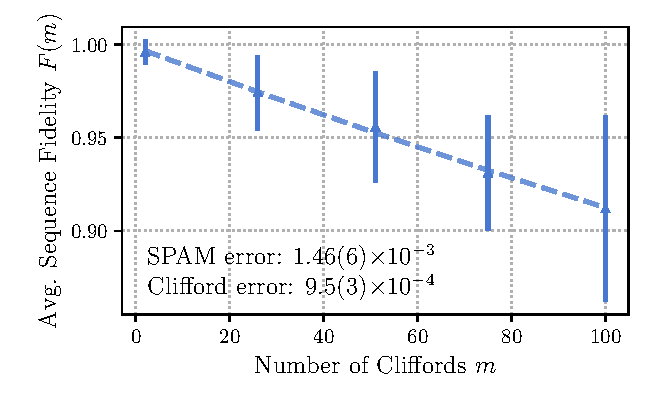
\includegraphics[width=0.75\linewidth]{
            figures/pdf_figure/rbm_fit.pdf
            }
        \end{center}
        \caption{
            Estimating single qubit Clifford fidelities, $F$, and SPAM errors using randomised benchmarking. 
            The data points are the average survival population after applying a sequence of $m$ random Clifford gates, and a final inverting Clifford gate. The dashed line is the fit to the decay model given by equation~\ref{eq:RBM_decay}. The error bars are given by the standard deviation of the survival populations.
            }
        \label{fig:rbm}
    \end{figure}

    High fidelity unitary operations (gates) are essential for both near
    intermediate scale quantum computing and for reducing overheads in required
    physical qubits and operations in fault-tolerant
    schemes~\cite{steane_overhead_2003}. To evaluate the quality of both our
    state-preparation and single qubit rotations, randomized benchmarking
    (RBM)~\cite{knill_randomized_2008, magesan_scalable_2011} is employed.  RBM consists of
    applying random combinations of a discrete set of gates to
    estimate an average error per gate.  The single-qubit Clifford
    group is chosen as the set of gates to evaluate. The single-qubit Clifford group is
    the set of unitaries which map the Pauli matrices to one another through
    conjugation. This can be thought of as the complete set of rotations of the
    Bloch sphere such that all valid combinations of the axis $(x \rightarrow
    \{\pm x,~\pm y,~\pm z\}),~(y \rightarrow \{\pm x,~\pm y,~\pm z\}),~(z
    \rightarrow \{\pm x,~\pm y,~\pm z\})$ are realized. There are 24 unitaries
    in this set. The RBM protocol is described in the
    thesis~\cite{hughes_benchmarking_2021}.
    First the qubit is prepared in some known initial state, i.e. prepared in
    some chosen basis. A gate sequence is then applied which consists of
    multiple random Clifford gates followed by a final `inverting' Clifford,
    where the `inverting' Clifford is chosen such that the full sequence
    performs the identity operation. The state is then measured in the same
    basis to find any deviations from the identity being performed due to gate
    errors. This is repeated with the same preparation and sequence multiple
    times to calculate the probability that the identity was performed --- thus
    giving the sequence fidelity. These steps are repeated for many different
    random sequences with a range of sequence lengths. The decay model used to find 
    the fidelity versus number of Clifford gates is given by\cite{hughes_benchmarking_2021},

    \begin{equation}
    \label{eq:RBM_decay}
        \mathcal{F}(m) = \frac{1}{2}\left( 1+(1-2\epsilon_{SPAM})(1-2\epsilon_c)^m\right),
    \end{equation}

    \noindent where $\mathcal{F}(m)$ is the fidelity of the sequence of length $m$,
    $\epsilon_{SPAM}$ is the state-preparation and measurement error, and
    $\epsilon_c$ is the average error per Clifford gate.  The Clifford gates are decomposed into
    sequences of $\pi/2$ and $\pi$ pulses about either the $x$- or $y$-axes. Up to $m=100$ Clifford gates are probed, and the decay of the fidelity, $\mathcal{F}(m)$, is fitted using the above model.
    The error per Clifford is found to be $\epsilon_c = 9.5(3) \times 10^{-4}$,
    while the SPAM error is $\epsilon_{SPAM} = 1.46(6) \times 10^{-3}$. The decay plot for
    this RBM sequence can be seen in figure~\ref{fig:rbm}. The error bars
    are given by the standard deviation of the survival populations. There are on average 3.50 $\pi/2$ pulses per Clifford, with a typical $\pi/2$ duration of $1.3~\mu$s.\\


\section{Motion}
\label{sec:Motion}
% Main points:
    % Quote characterisation method and values for various motional measurements.
    % Highlight where we are not yet at the capability we need.
    % State what improvements we plan to add.
% Pre reqs:
    % Motivation for control of motion of ion
    % Trap RF DC
    % Laser systems
    \mccorrect{XXX want a short introduction to the motion of the ion, and why we want to control it here. Describe what oscillators we have access to (like with quadrupole transitions).}

\subsection{Cooling}
\label{sec:Cooling}
% Main points:
    % Introduce why we want to cool
    % Doppler cooling
    % Sideband cooling
% Pre reqs:
    % Motional mode and beam geometry
    % Laser systems 
    % Trapping

    For any interaction involving the motion of the ion, we require both the
    ability to prepare and measure the motional state with high fidelity. For
    entangling gates, and the creation of squeezed states, which we 
    consider in this thesis (although as yet unwritten), it is assumed that the motional state is prepared in Fock state $|0\rangle$. The initially trapped ions will
    be in some unknown high temperature thermal state. To motionally prepare these ions, first Doppler cooling is applied, and then
    subsequently, pulsed sideband cooling. \\

\subsubsection{Doppler Cooling}
% Main points:
    % Quote final temperature reached (theory?)
    % Describe cooling parameters
% Pre reqs:
    % Motional mode and beam geometry
    % Laser systems 
    %XXX make more succinct.

    Doppler cooling relies on the fact that light incident on a moving ion will
    appear frequency shifted in the rest frame of the ion. For Doppler cooling
    of $^{40}$Ca$^+$, both the 397-nm and 866-nm lasers are applied. Initially the 397-nm laser is red
    detuned by $\sim$17.5~MHz. This results in the preferential
    absorption of a quanta of 397-nm light by ions with a velocity vector
    antiparallel to the photon k-vector. After this absorption, the ion will be in the
    excited $4P_{1/2}$ state and spontaneously decay to either $4S_{1/2}$,
    or $3D_{3/2}$ emitting a photon of either 397-nm or of 866-nm,
    respectively, into a random direction. The 397/866 decay paths have a branching
    ratio of 14.5~\cite{ramm_precision_2013}. As many photon kicks are required to cool the ions, the fluorescence cycle must be ``closed''. To prevent the electron from becoming trapped in the metastable $3D_{3/2}$ level, the 866-nm laser is applied on resonance.  The absorption and sequential emission of this 397-nm photon
    will lead to a net reduction in the motional energy of the ion if the emitted photon
    is higher energy than the photon absorbed. The equilibrium
    temperature is given by the condition where the Doppler cooling rate is
    equal to photon recoil heating of the ion. Assuming a Lorentzian absorption
    profile, the minimum temperature is given by,
    \begin{equation}
    T_{\rm Doppler} \approx \frac{\hbar\gamma}{2k_B},
    \end{equation}
    where $\hbar$ is the reduced Planck constant, $\gamma$ is the natural
    linewidth of the transition, and $k_B$ is Boltzmann's constant~\cite{}.\\ For
    $^{40}$Ca$^+$, the natural linewidth of the 397-nm transition is $\frac{\gamma}{2\pi} =
    21$~MHz, leading to a Doppler temperature of approximately 0.5~mK. Given a radial mode frequency of $\frac{\omega}{2\pi} = 4$~MHz, and the mean occupation number of the oscillator being given by,
    %[ref NIST https://www.physics.nist.gov/PhysRefData/Handbook/Tables/calciumtable4.htm] 
    \begin{equation}
        \bar{n} = \frac{1}{e^{\hbar\omega/k_B T}-1},
    \end{equation}
    the final thermal distribution is expected to have average phonon number $\bar{n} = 2.3$.
    %Using parameters summarised in table~\ref{tab:397_parameters}, we find practically the final temperature after Doppler cooling to be $\bar{n} \sim 5$, although further exploration into this discrepancy is needed.\\

\subsubsection{Sideband Cooling}
% Main points:
    % Quote final temperature reached
    % Describe SBC pulse sequence
    % We use a closed transition
% Pre reqs:
    % Motional mode spectra
    % Laser systems 
    % Rabi flopping

    \begin{figure}
        \begin{center}
        \noindent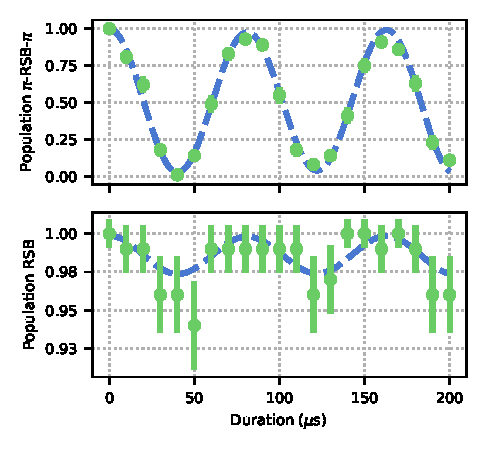
\includegraphics[width=0.75\linewidth]{
            figures/pdf_figure/sideband_thermometry.pdf
            }
        \end{center}
        \caption{
            Thermometry scan after Doppler and sideband cooling. The red points are the populations measured via on-resonance red sideband, RSB, pulses, and the blue points are the populations after a sequence of $\pi$-RSB-$\pi$ with varying RSB lengths. The dashed lines are fits to a thermal Fock state distribution, with truncation at Fock state = 100. The extracted mean occupation number is $\bar{n} = 0.03(1)$, and $\eta\Omega/(2\pi) = 73.1(4)$~kHz \mccorrect{XXX think this number is somehow wrong.}
            }
        \label{fig:SBC}
    \end{figure}

    %\noindent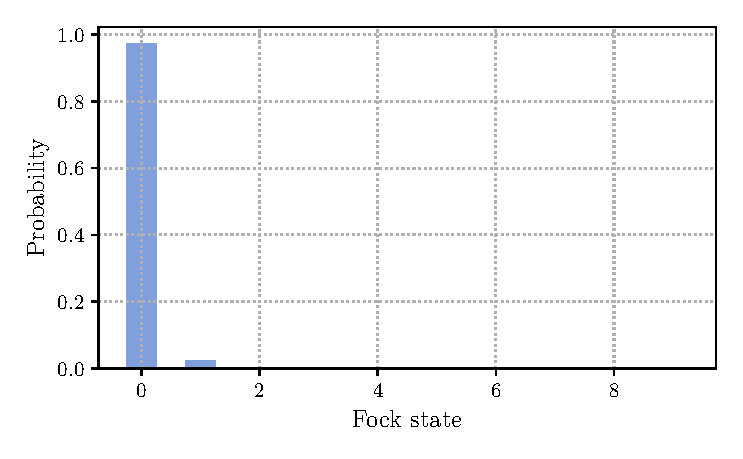
\includegraphics[width=0.75\linewidth]{
        %figures/pdf_figure/fock_state_distribution.pdf}


    To further cool the ions toward their motional ground state, resolved
    sideband cooling is used. The motion of the ion, described by a harmonic oscillator,
    modulates the transition frequencies of the ion, leading to sidebands at
    multiples of the motional frequency. For the $4S_{1/2} \leftrightarrow
    3D_{5/2}$ transition, at appropriate laser intensity and motional mode
    frequencies, these sidebands can be resolved spectroscopically. The pulsed
    sideband technique employed consists of red sideband pulses, followed by
    deshelving, and repumping pulses on the 854-nm and 866-nm transitions
    respectively. An example pulse sequence can be seen in
    figure~\ref{fig:sideband_cooling_sequence}, and experimental parameters used are summarised in table~\ref{tab:sbc_parameters}. \mccorrect{This pulse sequence and table is not yet made.}\\
    To verify the efficacy of our sideband cooling, thermometry
    experiments are performed by driving on resonance red sideband (RSB) and $\pi$-RSB-$\pi$ pulse
    sequences. The time dynamics of population flopping is measured as RSB
    pulse length is varied. In the case of Fock state $|0\rangle$, there should be full contrast 
    RSB oscillations, and no visible oscillations on the $\pi$-RSB-$\pi$ pulse. A thermal
    Fock state distribution (with truncation at Fock state = 100) is fitted to these
    signals to extract the mean occupation number, and $\eta\Omega$, the carrier
    Rabi frequency multiplied by the Lamb-Dicke parameter. A typical thermometry
    scan after Doppler and sideband cooling can be seen in
    figure~\ref{fig:SBC}. The mean occupation
    number after sideband cooling is found to be $\bar{n} = 0.03(1)$, and $\eta\Omega =
    XX$~MHz.\\
    Optimisation of the cooling parameters can be roughly performed by fitting
    temperature while scanning RSB $\pi$-pulse durations, total number of pulses,
    repumping and deshelving times. One can optimise for minimum temperature,
    however it is also important to optimise for total cooling duration. For
    single ion, single mode experiments, this duration is often not a limiting factor for experimental run-times,
    however for multi-ion crystals, any interaction involving the motion may
    require the sequential sideband cooling of multiple motional modes. This can
    not be easily parallalised due to the requirement that the RSB $\pi$-pulse is
    performed near resonance to one of the motional sidebands. This sequential
    cooling strategy can be either limiting when heating and cooling rates are
    comparable, or lead to prohibitive data acquisition times.\\
    To mitigate this issue, other sub-Doppler cooling techniques with larger
    accepted mode frequency bandwidths may be employed. Examples are dark-resonance
    cooling~\cite{}, electromagnetically induced transparency (EIT) cooling~\cite{}, and
    Sisyphus cooling~\cite{}. These techniques are not yet implemented in our system,
    but will be likely additions once we move to larger ion crystals.\\

\subsection{Heating Rates}
\label{sec:Heating}
% Main points:
    % Quote motional heating rates for mode we use (have access to).
    % Describe heating model?
% Pre reqs:
    % Thermometry
    % Motional modes
    % Trap

    \begin{figure}
        \begin{center}
        \noindent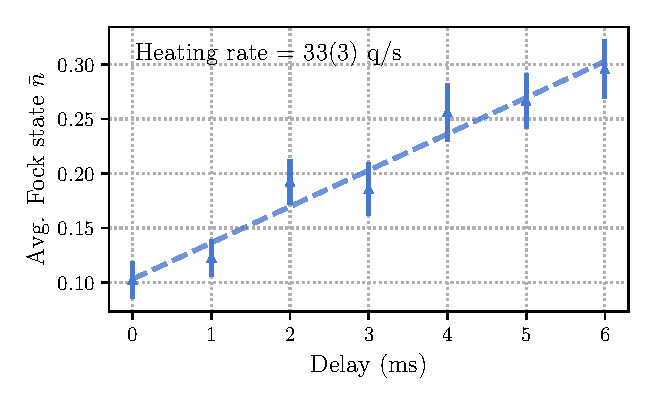
\includegraphics[width=0.75\linewidth]{
            figures/pdf_figure/heating_rate.pdf
            }
        \end{center}
        \caption{
            Heating rates of upper radial mode, measured by varying the delay between cooling and thermometry pulses. The dashed line is a linear fit to the data, with slope $33(3)$~quanta/s. The error bars are given by the standard deviation of the fitted $\bar{n}$.
            }
        \label{fig:heating rates}
    \end{figure}

    As mentioned, the cooling of the motional modes is only relevant if heating rates are acceptably low. Heating of the motion is predominantly caused by the ion trap
    itself~\cite{}. This can be due to imperfections in the surface of exposed
    dielectric and metals causing stray fields, or can be due to noise on the DC
    and RF drive voltages~\cite{}. Noise due to the surface of the trap can be
    mitigated by increasing ion-electrode distances, or by using traps with
    smaller surface area direclty exposed to the ion~\cite{}. In our case, as mentioned
    in sections~\ref{sec:The Ion Trap}, the \emph{NPL} trap has an ion-electrode 
    distance somewhat larger than most surface traps, but less than that of a
    macroscopic blade or rod style trap. To verify the heating rate of the
    system, a series of thermometry experiments were performed whilst varying the delay
    time between cooling and thermometry pulses. A typical plot can be seen in
    figure~\ref{fig:heating rates}. The heating rate of the system
    was found to be $33(3)$~quanta per second on the upper radial 4~MHz mode on
    one ion.\\
    %It is expected that the heating rate will be larger for lower frequency
    %motional modes if electric field noise is assumed to be uniform over its spectrum~\cite{}. 
    
    %We also verify
    %this by looking at heating rate on the radial mode while varying the axial
    %mode frequency. This is a useful diagnostic to check for unexpected heating
    %at certain frequencies, perhaps due to RF noise in the lab. We find....\\

\subsection{Motional Mode Stability}
\label{sec:Motional Mode Stability}
% Main points:
    % Quote motional mode drift 
    % Explain why it is currently drifty
    % Outline how this will be improved with the squareatron
% Pre reqs:
    % Trap

    \begin{figure}
        \begin{center}
        \noindent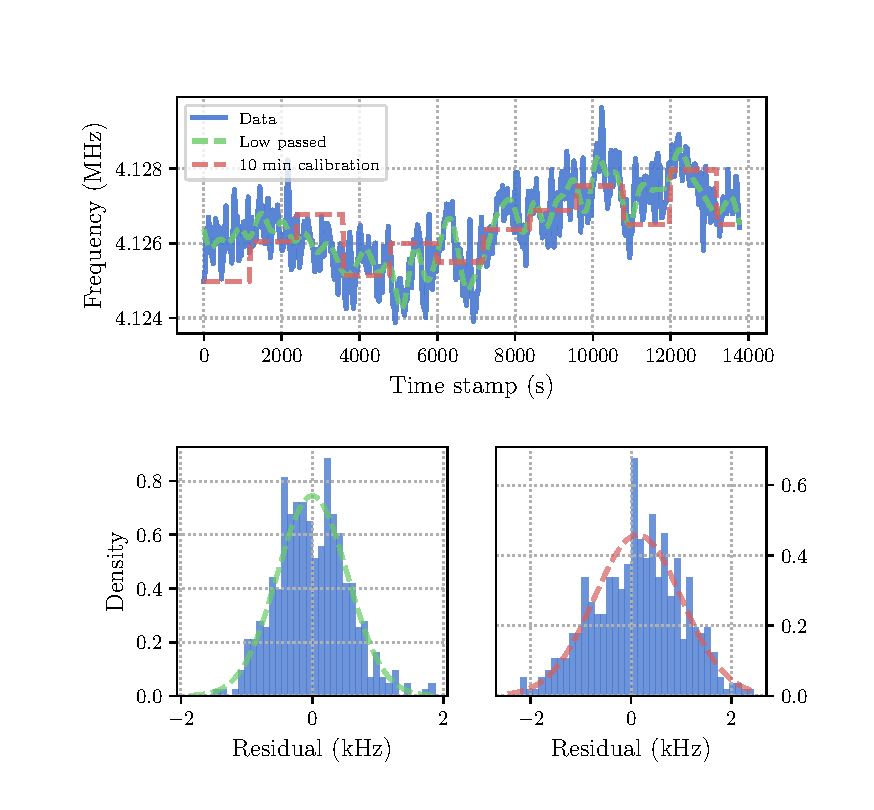
\includegraphics[width=\linewidth]{
            figures/pdf_figure/mode_drift.pdf
            }
        \end{center}
        \caption{
            \textbf{a)} Motional mode frequency drift over time. The radial motional mode frequency is measured by performing a ``tickle'' experiment. The resulting frequency trace is shown in blue. The green line shows a low pass filter of the data, with cut-off frequency of 1.67~mHz, corresponding to an assumed 10 minutes slow thermal drift. The motional mode frequency is typically calibrated every 10 minutes, which is indicated by the red line. 
            \textbf{b)} Residuals from the measured data and the low passed trace. The standard deviation of these residuals are due to ``fast'' noise which will likely not be elimated by either adding a slow active feedback loop on the RF amplitude or further isolating the resonator from temperature fluctuations. \mccorrect{XXX replace with box data.}
            \textbf{c)} Residuals from the measured data and expected calibrated mode frequencies. The standard deviation of these residuals suggests the typical misset detuning of the mode frequency in current experiments.
            }
        \label{fig:mode drift}
    \end{figure}

    Due to thermal drifts and microphonics introducing amplitude and frequency noise on the RF chain, drifts of the radial motional mode frequencies are seen over time. As will be discussed in the following section~\ref{sec:Motional Coherence}, this can lead to dephasing of the motional state. Here the current motional mode stability is characterised, possible causes are explained, and improvements are suggested. \\
    To measure the motional mode frequency an RF ``tickle'' experiment~\cite{} is performed. A short pulse of RF is applied to one of the trap DC electrodes which has a non-zero electric field projection to the mode we wish to probe. The tickle RF is scanned around the expected motional mode frequency, and when resonant, causes motional heating. This resonance is measured by observing an increase in fluorescence counts on a far red-detuned 397-nm transition. This measurement is repeated every 20 seconds, and the mode frequency is plotted over multiple hours. A typical plot can be seen in figure~\ref{fig:mode drift}. \mccorrect{XXX want to change this figure for the drifts with the box over the resonator.} Assuming that in normal operating conditions the mode frequency is calibrated every 10 minutes, a standard deviation of $\sigma/(2\pi) = 870$~Hz is found. As the frequency drift cannot currently be probed over shorter time scales, we can not yet estimate the contributions of fast noise, such as microphonics, versus slower noise on thermal drift time scales. 
    
    % Tracking noise source
    % Show resonator scan
    % Explain we sit either on peak or edge
    % show mode drift of +- edge of resonator.
    % This suggests amplitude drift
    % XXX However, we can distinguish between amplitude or resonator frequency drifts by changing the trap RF frequency. Figure~\ref{fig: mode drift} shows the motional mode frequency versus the trap RF frequency. The quadratic responce seen is due to the bandwidth of the resonator. By probing two points If the central frequency of the resonator drifts over time
    

\subsection{Motional Coherence Times}
\label{sec:Motional Coherence}
% Main points:
    % Quote measured result for motional coherence time
    % Give estimate for what times we need for future experiments
    % Give estimate contributions from motional heating and from mode instability
    % What fix will we do for improving this - squareatron from prev section, resonator.
% Pre reqs:
    % Trap RF
    % Trap Resonator
    % Motional mode stability
    % SBC
    We will utilise the motional modes of the ion to store quantum information.
    As with the section on spin coherence times~\ref{sec:Coherence}, the
    fidelity of operations, and success probability of algorithms will be
    limited by the coherence time of the motional state.  To measure motional
    coherence, a Ramsey sequence is performed between states $|\downarrow, 0
    \rangle$ and $|\downarrow, 1 \rangle$, where the first element is the qubit
    state, and the second element is the motional Fock state. To prepare these
    states the following pulse sequence is applied:
    \begin{itemize}
    \item State prepare system to $|\downarrow, 0\rangle$ via optical pumping and sideband cooling.
    \item Apply $\pi/2|_y$-pulse on carrier transition to prepare the qubit in $(|\downarrow, 0\rangle + |\uparrow, 0\rangle)/\sqrt{2}$.
    \item Apply $\pi$-pulse on the RSB to prepare the motional state in $(|\downarrow, 0\rangle + |\downarrow, 1\rangle)/\sqrt{2}$.
    \end{itemize}
    The full Ramsey sequence is then completed by delaying for some time $t$,
    and then reversing the above state prep and measuring spin population in
    $|\downarrow\rangle$. \\
    There are two main mechanisms for motional decoherence: motional heating, as
    characterised in section~\ref{sec:Heating}, and motional dephasing due to
    mode frequency instability, as discussed above. \\
    A heating rate dominated coherence time is given by, $\tau_{\rm HEAT} =
    (\sqrt{e}-1)/\dot{\bar{n}}$~\cite{}, where $\dot{\bar{n}}$ is the heating
    rate. A dephasing dominated coherence time, consisting of the
    motional mode frequency drifting shot-to-shot with a standard deviation
    $\sigma_{\omega}$, is characterised by a Gaussian decay profile with a coherence time
    of $\tau_{DEPH} = \sqrt{2}/\sigma_{\omega}$.\\
    Evaluating both of these models with $\dot{\bar{n}}=33(3)$~q/s, and
    $\sigma_{\omega}/(2\pi) = 750$~Hz, the expected motional coherence times of $\tau_{\rm
    HEAT} \approx 20$~ms and $\tau_{\rm DEPH} \approx 0.3$~ms respectively, are found. From these auxiliary characterisations of the motional modes, it is expected that the coherence time will be limited by motional dephasing.  However, as can be
    seen in figure~\ref{fig:motional_coherence}, a
    motional coherence time of XX(X)~ms is found experimentally by fitting a Gaussian decay. \mccorrect{XXX Figure not yet added. I want to retake motional coherence scan with the box over the resonator.} \\
    Assuming this was dominated by motional mode drifts between shots, the motional mode drift can be estimated to have a standard deviation, $\sigma_{\omega}/(2\pi) =
    225$~Hz. Comparing this to the previously measured long-term motional mode
    stability, we see a discrepancy. This is likely due to the issue of time
    scales. The motional mode stability in the described Ramsey experiment is
    only relevant over the time it takes to collect enough statistics for one
    fringe scan, around 1 second. However, the above motional mode stability is
    probed only every 20 seconds and so may overestimate the instability over
    shorter time scales.\\ 
    %Work must be done to estimate the fast motional
    %noise, however, first there may be simple improvements that can be made to
    %the RF chain to improve both short and long term motional mode stability.
    %These improvements are described in section~\ref{sec:Trap RF Chain}.\\


\section{Spin-Dependent Forces}
\label{sec:Spin-Dependent Forces}
% Main points:
    % This is a primitive for motional control
    % This (we will see), is functionally a primitive for two qubit spin entanglement
    % Show equation as quite key to future work
% Pre reqs:
    % Motional mode spectra
    % 729 system
    % AOM control of 729
    For full control of the spin-motion hybrid system, we require interactions
    that couple the two. Perhaps the simplest of this class of interactions
    are the red- and blue-sidebands (RSB and BSB respectively). The  RSB
    interaction was used previously in the thermometry and sideband cooling
    sections~\ref{sec:Cooling}. The RSB (BSB) consists of a single frequency
    laser tuned at the carrier frequency minus (plus) the motional mode frequency,
    $\omega_m$. The interaction is well described by the (Anti-) Jaynes-Cummings
    Hamiltonian, and effectively couples spin flips with the addition or
    subtraction of a motional quanta depending on the initial spin state. Here,
    another such interaction coupling spin and motion, known as the
    spin-dependent force, SDF, is introduced. If the RSB and BSB interactions couple spin-motion in
    the motional Fock basis, then the SDF couples the two in a
    motional coherent basis. The SDF displaces the motional state in phase
    space, with a direction dependent on the spin state and an effective detuning parameter.\\
    The optical Mølmer-Sørensen (MS) scheme~\cite{} is used to generate the
    SDF via a bichromatic laser field. Bichromatic refers to the simultaneous
    application of two tones symmetrically detuned around the qubit carrier
    frequency, with absolute detuning approximately equal to the motional mode
    frequency, $\delta \approx \omega_{m}$. The resulting interaction, when
    ignoring off resonant and higher order couplings, is given by,
    \begin{equation}
        \hat{H}_{MS} = \hbar \eta\Omega~\hat{\sigma}_\phi\cos(\delta t) \left( \hat{a} e^{-i\omega_{m} t} + \hat{a}^\dagger e^{i\omega_{m} t} \right),
    \end{equation}
    where $\eta$ is the Lamb-Dicke parameter, $\Omega$ is the carrier Rabi
    frequency, $a(a^\dagger)$ is the lowering (raising) operator, and
    $\hat{\sigma}_\phi$ is the Pauli operator with $\phi$ being in the $x$-,~$y$-plane.
    Applying the rotating wave approximation, and defining $\delta_g = \delta -
    \omega_{m}$, the interaction Hamiltonian can be approximated
    to,
    \begin{equation}
        \hat{H}_{MS} \approx \frac{\hbar \eta\Omega}{2}~\hat{\sigma}_\phi \left( a e^{-i\delta_g t} + a^\dagger e^{i\delta_g t} \right).
    \end{equation}
    The trajectory of this displacement can be controlled by varying $\delta_g$: on
    resonance, $\delta_g = 0$, corresponds to linear trajectories, whilst off resonance,
    $\delta_g \neq 0$, corresponds to cyclic trajectories where after some time $t =
    2\pi/\delta_g$, the motion returns to the initial state (with perhaps some phase shift). 
    This control is exploited in both two-qubit entangling gate experiments, as well as
    in the creation of squeezed states.\\

\subsection{Calibrating the SDF}
% Main points:
    % Here describe what error sources "look like"
    % Describe detuning and duration scans
    % Describe how we can detect these errors via the above strategy. Refer to OB thesis.
    % Fit an SDF with the errors?
% Pre reqs
    % Motional mode spectra
    % 729 system
    % AOM control of 729

    \begin{figure}
        \begin{center}
        \noindent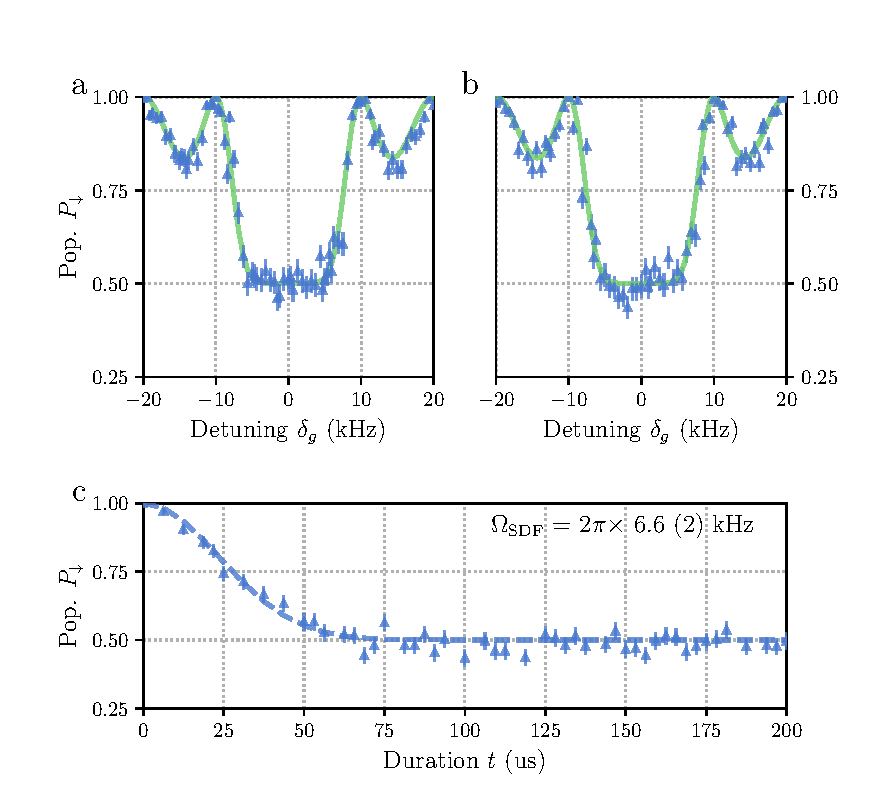
\includegraphics[width=\linewidth]{
            figures/pdf_figure/sdf.pdf
            }
        \end{center}
        \caption{
            SDF traces. \mccorrect{XXX need to update figure with legend and add caption.}
            }
        \label{fig:SDF}
    \end{figure}

    The MS interaction is widely used in ion trap experiments due to it being robust against varying intial motional states, and to the effects of heating during the pulse sequence. However, in our use case, the SDF is sensitive to various frequency and power miscalibrations and drifts of these between calibrations.  Here we describe briefly the work flow for calibrating and optimising the SDF behaviour.\\
    In honesty, there are not many moving parts in the SDF interaction, we must calibrate the central qubit frequency, the motional mode frequency, the power in each tone, and the durations of the pulses. Complications come from the reality that the ion is a multi-level system, posseses multiple motional modes, and that experimentally each parameter can only be controlled to a certain precision.\\
    The effect of nearby motional modes is negated by either selecting the
    interaction mode to be well seperated from the others either in frequency, by beam geometry, by
    operating the SDF near to resonance of the desired mode, or by using pulse
    shaping to ramp the power of the SDF and suppress the off-resonant
    excitation of these other modes~\cite{}. There are many tricks to either mitigate or
    exploit the effects of these other modes~\cite{}, and we will not go into detail
    here. \\
    The power balance of the SDF tones is complicated due to our use of AOMs.
    AOMs generate frequency shifts in the laser beam at the expense of small
    frequency-dependent angular shifts. After the AOM, the beam is coupled into a
    single mode fibre (see figure~\ref{fig:729}), and so the AOMs effectively introduce a
    frequency-dependent loss. To calibrate the power balance, a pick
    off of the bichromatic beam before the ion is monitored on a high bandwidth photodiode.
    The beatnote contrast is measured for the two tones and the power
    balance is optimised by maximising this contrast.\\
    The far off-resonant levels of our ion lead to light-shifts of our qubit
    frequency. Practically to account for the light-shift the central qubit frequency must be calibrated at the
    optical power used for the interaction. This is done with the SDF interaction
    itself. When the qubit frequency is set incorrectly, the two tones will no
    longer have the same absolute detuning from their respective RSB or BSB.
    This manifests as a ``skewness'' of the SDF detuning trace. By varying the qubit frequency and
    inspecting these detuning scans, the desired SDF behaviour can be found. \\
    To verify the behaviour of the calibrated SDF, the experimental data is compared with theory. Both
    ``detuning'' and ``duration'' scans are used. The ``detuning'' scan is performed by
    varying the detuning, $\delta_g$, of the interaction, whilst keeping the
    SDF duration, $t$, constant, and vice-versa for the ``duration'' scan. \\
    Figure~\ref{fig:SDF} $c$ shows the measured duration scan with a fit~\cite{} given by,
    \begin{equation}
        P_{\downarrow,\mathrm{th}} = \frac{1}{2} \left[ 1 + e^{-4\left( \bar{n} + \frac{1}{2} \right) |\alpha(t)|^2} \right],
    \end{equation}
    %from Burd thesis, equation 3.30.
    where it is assumed that the motional state is thermal with average Fock state $\bar{n}
    = 0.03(1)$ which is found previously from thermometry measurements. Here the
    displacement, $|\alpha(t)| = \Omega_{\rm SDF} t/2$, where $\Omega_{\rm SDF}$ is the
    SDF amplitude. 
    \mccorrect{XXX need to populate the following experimental values.}These measurements were performed with a duration of XX~ms, total power of xx~mW, $\delta_{\rm LS}=2\pi\times XX$~kHz.
    We find $\Omega_{\rm SDF} = 2\pi\times 6.6(2)$~kHz, from the
    measured fit, which is in good agreement with the expected value of
    $\Omega_{\rm SDF} = \eta\Omega_{\rm CAR}$, where Lamb-Dicke parameter $\eta =
    0.05$XXX and $\Omega_{\rm CAR} = 2\pi \times 132$~kHz XXX measured from Rabi
    flopping at 15XXX mW.\\
    The detuning scan, shown in figure~\ref{fig:SDF} $a$, is fitted by taking the
    displacement to be $|\alpha(t)| = \Omega_{\rm SDF} \sin(\delta t/2)/\delta$. Here,
    a qualitatively good agreement between the measured data and the
    expected behaviour is seen, with the main features being the ``closure''
    at $\delta = 2\pi/t$ where the motional state returns to the initial state,
    and the central flat region around $P_{\downarrow, \mathrm{th}} =0.5$ where
    the two motional wave packets are non-overlapping.\\
    \mccorrect{XXX need to add description of detuning scan $b$, where tone balance is inccorect.}
    % find $\Omega_{SDF} = 2\pi\times 6.3(2)$~kHz, fitted with $\bar{n} = 0.03$.


\section{Two-Qubit Entangling Gates}
\label{sec:Two-Qubit Entangling Gates}
% Main points:
    % Intro/brief outline of goal of two-qubit gate. Truth table? Preparing in Bell state. This is tool kit for spin control of our system.
    % Discuss likely limitations being nearby hot motional modes, no pulse ramping
    % Current error vs what we expect we need for future experiments.
    % Here empasise that the SDF we discuss previously can be used to generate entanglement.
    % Showing phase coherence between operations is nice here.
% Prereqs:
    % SDFs
    % Single qubit gates
    % What available transitions we have
    % Motional mode spectra

    \begin{figure}
        \begin{center}
        \noindent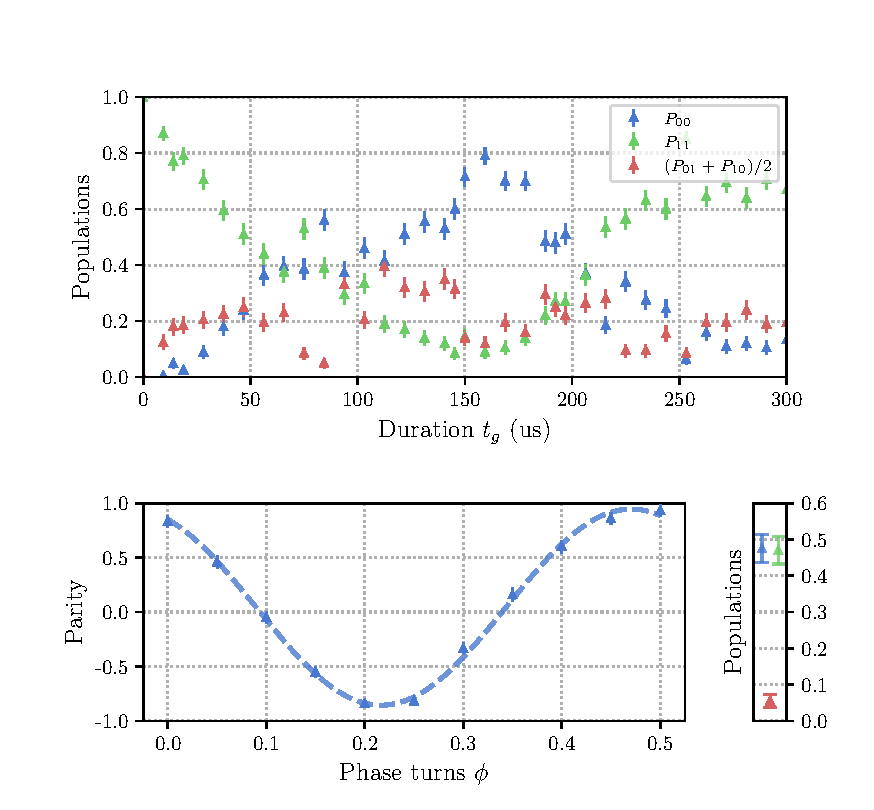
\includegraphics[width=\linewidth]{
            figures/pdf_figure/ms_gate.pdf
            }
        \end{center}
        \caption{
            Experimental data for $\mathcal{F}=92(2)$\% Mølmer-Sørensen (MS) two-qubit entangling gate.
            \textbf{a)} Populations versus duration scan of the MS interaction.
            Each point corresponds to the average of 200 shots, and the error
            bars are given by the standard deviation of these averages. The blue
            points are the populations of both ions being in the $|0\rangle$
            state, $P_{00}$, the green points are the populations of both ions
            being in the $|1\rangle$ state, $P_{11}$, and the red points are the
            ions being the the opposite states, $(P_{01}+P_{10})/2$. The desired
            entangling gate corresponds here to $t =  75~\mu$s. 
            \textbf{b)} Parity oscillations after the MS interaction. The parity
            is defined as $P_{00} + P_{11} - P_{01} - P_{10}$. The fitted
            contrast here is $0.90(2)$.
            \textbf{c)} Populations at the desired entangling gate time, $t =
            75~\mu$s.  
            }
        \label{fig:ms_gate}
    \end{figure}

    We perform two-qubit entangling gates using the Mølmer-Sørensen (MS)
    interaction~\cite{}. This interaction is the same described SDF from the
    previous section, but applied globally to two ions. The MS interaction
    relies on the spin dependent geometric phase accumulated during the motional
    displacement~\cite{ozeri_tutorial_2011}. To create a two-qubit entangled state, a differential
    geometric phase of $\pi/2$ must be accumulated between the two-qubit basis
    states. To ensure there is no residual motional entanglement, the final
    motional state must return to the initial state. In practise, using an SDF
    detuned by $\delta_g$, this is achieved by applying the MS interaction for a
    time $t = 2\pi/\delta_g$. The MS gate is a universal two-qubit gate, and
    along with only single qubit gates, constitutes a universal gate set for
    discrete quantum algorithms.\\  
    Here we quote the current fidelity of experimentally demonstrated two-qubit gates on
    our system. The fidelity serves to quantify the similarity of
    two density matrices~\cite{}.  For the use case of quantum information processing, what we
    care about is that the experimental unitary applied in the gate sequence closely resembles the unitary we desire theoretically. In general this
    means that the fidelity of the applied unitary should be measured in an input
    state agnostic way. Unfortunately, this is often not practical as the input
    state space can be unwieldly, and the act of preparing the input state can
    also be error prone. As a compromise, the unitary is tested with either
    one, or a set of input states, and the fidelity of the output state
    is measured with respect to the known target state. If the error mechansisms of the 
    unitary are well understood, arguments can be made that this measured
    fidelity for a set of input state is representative (or not representative)
    of the average fidelity over the input state space~\cite{}.\\
    Here for a two-qubit entangling gate, we target the creation of the Bell
    state $|\Phi^+\rangle = 1/\sqrt{2} \left( |00\rangle +
    e^{i\phi_0}|11\rangle \right)$, from an initial state of $|00\rangle$.
    The fidelity between our mixed state $\rho$, and the pure Bell state may be
    given by,
    \begin{equation}
        \mathcal{F} = \langle \Phi^+ | \rho | \Phi^+ \rangle = \frac{1}{2} \left( \rho_{00,00} + \rho_{11,11} \right) + \frac{1}{2}\left( e^{i\phi_0}\rho_{11,00}+e^{-i\phi_0}\rho_{00,11}\right),
        \label{eq:Fidelity}
    \end{equation}
    To extract the fidelity experimentally, the popular
    protocol~\cite{}, is followed where the first bracketted term of
    equation~\ref{eq:Fidelity} is measured by performing projective measurements
    of the two ions after the gate sequence to extract populations, and the second bracketted term,
    known as the coherence terms, are measured by applying a global analysis
    $\pi/2|_\phi$ pulse to the two ions and applying parity measurements. \mccorrect{XXX define parity measurements.} The
    contrast of the parity oscillations when varying the phase $\phi$ of the
    $\pi/2$ pulse yields the desired coherence term magnitude and phase. The creation of a Bell state is required for two qubit entangling, however, it does not matter what basis this Bell state is in, as long as it is consistent between experiments, and so the target Bell state phase may be floated. Practically this is equivalent to taking only the magnitude of the fitted parity oscillations for calculating the final fidelity, and ignoring the phase offset.\\
    The best two-qubit entangling gate fidelity currently achieved on our system is $\mathcal{F}=92(2)\%$. As shown in figure~\ref{fig:ms_gate}, the magnitude of the parity scan was measured to be 0.90(2), while the populations $\left( \rho_{00,00} + \rho_{11,11} \right) = 0.95(2)$. Each population point in these figures are found by taking the average of 200 shots of the gate sequence.\\

    These results serve as both a proof of principle for full spin control on
    our system, but also as a benchmark to which we can compare future system
    improvements.  For future work, we will require the use of this entangling
    gate either as Bell state preparation for input to analogue simulation
    experiments~\cite{}, or as a primitive gate for the spin component of hybrid
    algorithms~\cite{}.  In both these cases, especially any use that requires
    multiple concatenated entangling gates, we will likely require improved gate
    fidelities. It is suspected that the current fidelities are limited by nearby hot
    motional modes, and the lack of pulse shaping in the gate sequence. We
    expect that with the addition of pulse shaping, 
    the effect of nearby off-resonant transitions will be greatly suppressed, and by sideband cooling of
    nearby motional modes, contributions from unwanted
    spin-motion couplings will be negated.\\
